\documentclass[../main.tex]{subfiles}
\begin{document}
\section*{\textbf{\underline{Section name:} Exterior angle property of a triangle}}

\begin{enumerate}
    \item Draw a triangle.
        \begin{center}
        \begin{minipage}{0.4\textwidth}
        \begin{enumerate}[label=\roman*., leftmargin=*]
            \item Number of sides $\ans{1cm}{3}$
            \item Number of angles $\ans{1cm}{3}$
            \item Number of vertex $\ans{1cm}{3}$
        \end{enumerate}
        \end{minipage}
        \end{center}
        \hspace{1cm}
    \item Mark the interior angles of triangles as A, B, C and exterior angles as X, Y, Z.
        \begin{center}
			\begin{tikzpicture}
                \triangleDiagram[0][0][4][0][2][3]
			
				\extendArrow{B}{A}{1.5}{Y}
                \extendArrow{A}{C}{1.5}{X}
				\extendArrow{C}{B}{1.5}{Z}
				
                \markAngle{\textbf{\textcolor{green!70!black}{C}}}{B}{C}{A}
                \markAngle{\textbf{\textcolor{green!70!black}{B}}}{A}{B}{C}
                \markAngle{\textbf{\textcolor{green!70!black}{A}}}{C}{A}{B}
                \markAngle{\textbf{\textcolor{green!70!black}{Y}}}{Y}{A}{C}
                \markAngle{\textbf{\textcolor{green!70!black}{X}}}{X}{C}{B}
                \markAngle{\textbf{\textcolor{green!70!black}{Z}}}{Z}{B}{A}
				
			\end{tikzpicture}
		\end{center}
        \hspace{1cm}
    \item Answer the following based on exterior angle property of triangle.\\[1cm]
           \noindent
        	\begin{minipage}[t]{0.3\textwidth}
        		\begin{tikzpicture}
                \triangleDiagram[0][0][3][0][1.5][3]
				
				\extendArrow{B}{A}{1.5}{Y}
				\extendArrow{A}{C}{1.5}{X}
				\extendArrow{C}{B}{1.4}{Z}
				
                \markAngle{C}{B}{C}{A}
                \markAngle{B}{A}{B}{C}
                \markAngle{A}{C}{A}{B}
                \markAngle{X}{X}{C}{B}
                
			\end{tikzpicture}
               \centering
                X=$\ansqus{A}{B}$
        	\end{minipage}
        	\hfill
        	\begin{minipage}[t]{0.3\textwidth}
        		\begin{tikzpicture}
                \triangleDiagram[0][0][3][0][1.5][3]
				
				\extendArrow{B}{A}{1.5}{Y}
				\extendArrow{A}{C}{1.5}{X}
				\extendArrow{C}{B}{1.4}{Z}
				
                \markAngle{C}{B}{C}{A}
                \markAngle{B}{A}{B}{C}
                \markAngle{A}{C}{A}{B}
                \markAngle{Y}{Y}{A}{C}
                
			\end{tikzpicture}
            \centering
                Y=$\ansqus{B}{C}$
        	\end{minipage}
        	\hfill
        	\begin{minipage}[t]{0.3\textwidth}
        	\begin{tikzpicture}
                \triangleDiagram[0][0][3][0][1.5][3]
			
				\extendArrow{B}{A}{1.5}{Y}
                \extendArrow{A}{C}{1.5}{X}
				\extendArrow{C}{B}{1.4}{Z}
				
                \markAngle{C}{B}{C}{A}
                \markAngle{B}{A}{B}{C}
                \markAngle{A}{C}{A}{B}
                \markAngle{Z}{Z}{B}{A}
                
			\end{tikzpicture}\\
            \centering
                Z= $\ansqus{A}{C}$
        	\end{minipage}
    \newpage
    \item Identify the unknown angles.\\
		\noindent\begin{minipage}[t]{0.3\textwidth}
			\begin{tikzpicture}
				\triangleDiagram[0][0][4][0][2][3]
				
                \extendArrow{A}{C}{1.3}{X}
                
                \markAngle{$60^\circ$}{A}{B}{C}
                \markAngle{$60^\circ$}{C}{A}{B}
                \markAngle{X}{X}{C}{B}
                
			\end{tikzpicture}\\
			\centering
			\textbf{\textcolor{green!70!black}{X = 120$^\circ$}}
		\end{minipage}
		\hspace{0.5cm}
		\begin{minipage}[t]{0.3\textwidth}
			\begin{tikzpicture}
                \triangleDiagram[0][0][4][0][0][3]
                
                \extendArrow{A}{C}{1.3}{M}
				
                \markAngle{$45^\circ$}{A}{B}{C}
                \tkzMarkRightAngle[size=0.4](C,A,B)
				\tkzLabelAngle[pos=1.0](C,A,B){$90^\circ$}
                \markAngle{M}{M}{C}{B}
				
			\end{tikzpicture}\\
			\centering
			\textbf{\textcolor{green!70!black}{M = 135$^\circ$}}
		\end{minipage}
		\hspace{0.5cm}
		\begin{minipage}[t]{0.3\textwidth}
			\begin{tikzpicture}
                \triangleDiagram[0][0][5][0][1.5][3]
				
                \extendArrow{A}{B}{1.5}{P}
				
                \markAngle{$80^\circ$}{B}{C}{A}
                \markAngle{$55^\circ$}{C}{A}{B}
                \markAngle{P}{C}{B}{P}
                
			\end{tikzpicture}\\
			\centering
			\textbf{\textcolor{green!70!black}{ P = 135$^\circ$}}
		\end{minipage}\\
        [2cm]
        \begin{minipage}[t]{0.3\textwidth}
			\begin{tikzpicture}
                \triangleDiagram[1][0][4][0][0][3]

                \extendArrow{C}{A}{1.5}{Y}
				
                \markAngle{$25^\circ$}{A}{B}{C}
                \markAngle{$35^\circ$}{B}{C}{A}
                \markAngle{Y}{B}{A}{Y}
				
			\end{tikzpicture}\\
			\centering
			\textbf{\textcolor{green!70!black}{Y = 60$^\circ$}}
		\end{minipage}
		\hspace{0.5cm}
		\begin{minipage}[t]{0.3\textwidth}
			\begin{tikzpicture}
                \triangleDiagram[0][0][3][0][1.5][3]
				
                \extendArrow{B}{A}{1.3}{N}

                \markAngle{$75^\circ$}{A}{B}{C}
                \markAngle{$75^\circ$}{B}{C}{A}
                \markAngle{N}{N}{A}{C}
				
			\end{tikzpicture}\\
			\centering
			\textbf{\textcolor{green!70!black}{N = 150$^\circ$}}
		\end{minipage}
		\hspace{0.5cm}
		\begin{minipage}[t]{0.3\textwidth}
			\begin{tikzpicture}
                \triangleDiagram[1][0][4][0][5][3]
				
                \extendArrow{C}{A}{1.3}{Q}
				
                \markAngle{$35^\circ$}{A}{B}{C}
                \markAngle{$105^\circ$}{B}{C}{A}
                \markAngle{Q}{B}{A}{Q}
                
			\end{tikzpicture}\\
			\centering
			\textbf{\textcolor{green!70!black}{ P = 135$^\circ$}}
		\end{minipage}\\
		[2cm]
		\begin{minipage}[t]{0.3\textwidth}
			\begin{tikzpicture}
                \triangleDiagram[0][0][4][0][0][3]
				
				\tkzLabelPoint[below left](A){$B$}
				\tkzLabelPoint[below left](B){$A$}
				\tkzLabelPoint[below right](C){$C$}

                \markAngle{$45^\circ$}{A}{B}{C}
                \markAngle{$x$}{B}{C}{A}
                \tkzMarkRightAngle[size=0.4](C,A,B)
				\tkzLabelAngle[pos=1.0](C,A,B){$90^\circ$}
				
			\end{tikzpicture}\\
			\centering
			\textbf{\textcolor{green!70!black}{X = 45$^\circ$}}
		\end{minipage}
		\hspace{0.5cm}
		\begin{minipage}[t]{0.3\textwidth}
			\begin{tikzpicture}
                \triangleDiagram[0][0][4][0][5][3]
				
				\tkzLabelPoint[below left](A){$B$}
				\tkzLabelPoint[above](B){$A$}
				\tkzLabelPoint[below right](C){$C$}
				
                \markAngle{$X$}{A}{B}{C}
                \markAngle{$110^\circ$}{B}{C}{A}
                \markAngle{$38^\circ$}{C}{A}{B}
                
			\end{tikzpicture}\\
			\centering
			\textbf{\textcolor{green!70!black}{X=32$^\circ$}}
		\end{minipage}
		\hspace{0.5cm}
		\begin{minipage}[t]{0.3\textwidth}
			\begin{tikzpicture}
                \triangleDiagram[0][0][4][0][2][3]
				
				\tkzLabelPoint[below left](A){$B$}
				\tkzLabelPoint[above](B){$A$}
				\tkzLabelPoint[below right](C){$C$}
				
                \markAngle{$3x-15^\circ$}{A}{B}{C}
                \markAngle{$x+35^\circ$}{B}{C}{A}
                \markAngle{$2x+10^\circ$}{C}{A}{B}
				
			\end{tikzpicture}\\
			\centering
			\textbf{\textcolor{green!70!black}{ X = 25$^\circ$}}
		\end{minipage}
\end{enumerate}
\end{document}
